% Section 9 --- Agentic Timeline (compressed)

\section{From Measurement to Deployment: The Agentic Timeline}
\label{sec:agentic-timeline}

Industry is moving from minute-scale chat to hour-scale coding agents to
day-scale autonomous research agents, and the research literature has followed
by making duration the independent variable: reliability frameworks for agents
now substitute task duration for time and non-completion for failure
\citep{khanal2026reliability}, and long-horizon surveys report that outcome
signals lose information as the horizon grows \citep{chen2026horizongap}. This
section supplies the term those frameworks are missing --- what sets the
horizon at which an agent stops being reliable. At each new horizon a different sub-capability becomes load-bearing: T1.1 at chat (harness-patchable, \S\ref{sec:injection-tell}), T2.3 and T3.1 at hour-scale (agent must honour a budget and report progress truthfully), the full profile $(\parkinson, \CAR, \confab)$ at day-scale. Required calibration grows tighter with the horizon.

\begin{hypothesis}[Agentic Timeline]
\label{hyp:agentic-timeline}
$T_{\max}(A) \;\propto\; \frac{1}{\cce(A)} \cdot f(\CAR(A))$, with $f$ monotone-increasing in $\CAR$.
\end{hypothesis}

Combined with the empirics of \S\ref{sec:l2}--\ref{sec:l3}: L2 does not scale with capability, Reverse-Scaling grows $|\confab|$ with reasoning budget. \textbf{$T_{\max}$ scales with neither. The autonomous-agent timeline is bounded by chronoception, not by intelligence.}

\paragraph{Pre-registered P12 and HCAST support.}
On any horizon-stratified benchmark with $\geq 5$ horizon tiers, slope of success decay with $\log T$ scales as $-(1 - \CAR)$. On the METR HCAST corpus (14{,}709 runs after filtering, 20 frontier models), five reasoning models cluster at steeper mean $|\text{slope}| = 0.318$ vs.\ $0.264$ for fifteen non-reasoning models --- a $20\%$ effect at matched short-horizon success (Fig.~\ref{fig:p12-hcast}). The separation is statistically supported: Mann--Whitney $U = 58$, one-sided $p = 0.040$; permutation test ($20{,}000$ resamples, one-sided) $p = 0.037$; rank-biserial $r_{\text{rb}} = -0.55$ (large effect, reasoning stochastically dominates). We report one-sided because Theorem~\ref{thm:reverse-scaling} makes a directional prediction (reasoning models decay \emph{faster}, not just differently); the two-sided form is marginal ($p = 0.081$). Supportive at $\alpha = 0.05$; a strict $\CAR$-anchored quantitative P12 additionally requires direct T2.3 measurements on the HCAST panel, which we have not run.

\begin{figure}[h]
\centering
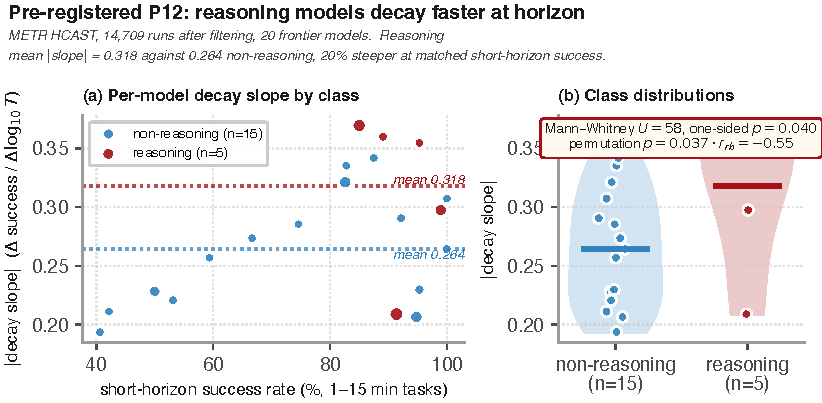
\includegraphics[width=\linewidth]{figures/p12_hcast.pdf}
\caption{P12 support on METR HCAST. Reasoning models cluster at steeper decay slopes despite competitive short-horizon success --- the L2 mechanism at the model-class level.}
\label{fig:p12-hcast}
\end{figure}

\citet{kwa2025metrhorizons} document horizon saturation empirically; we supply
a structural mechanism. Theorem~\ref{thm:reverse-scaling} says the corner-case
fix (more reasoning) makes it worse; the constructive fix
(wall-clock-supported loss) is the subject of Paper 2 (\textsc{ChronoStack}).

\paragraph{Why scaling out does not substitute.} The field's dominant response
to horizon limits is orchestration --- surveys of the long-horizon literature
find multi-agent coordination papers outnumbering work on the single-agent
loop by orders of magnitude \citep{chen2026horizongap}. Orchestration does not
install chronoception in any of the parts. A supervisor apportioning deadlines
across sub-agents is apportioning a resource none of them can perceive, and
aggregating progress reports none of them can ground: our panel measures
$\tself$ tracking the agent's own output length rather than the clock
(\S\ref{sec:limitations}), so a sub-agent reporting ``about two seconds'' is
reporting how much it wrote. Nor is there a model to route around the problem
to --- $\CAR \ll 1$ on all fourteen configurations from seven vendors. The
bound applies to the orchestrator as much as to the worker, and a blind spot
distributed across more agents is a blind spot multiplied.
